
\begin{figure}[t]
    \centering
    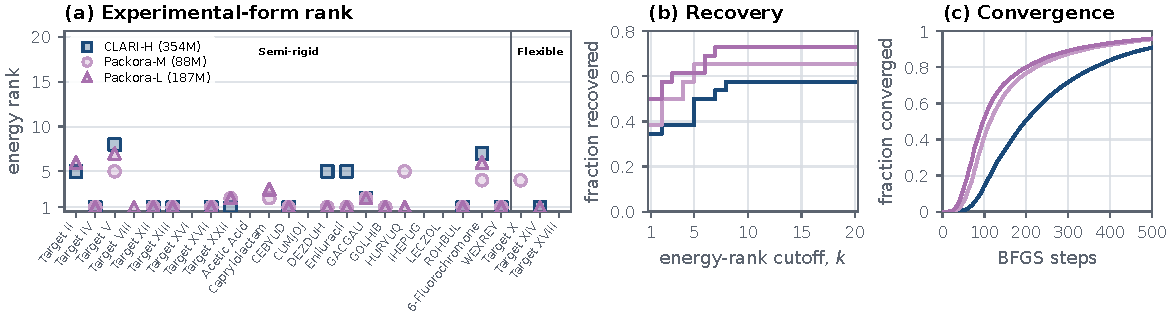
\includegraphics[width=\textwidth]{figures/generated/fig_fastcsp_single_ranking.pdf}
    \caption{\textbf{FastCSP single-polymorph benchmark.}
    We generate 1{,}000 candidates for each of the 26 targets, relax them with
    UMA-S-1.2~\citep{wood2025family}, and rank them by increasing energy.
    \textbf{(a)} Best energy rank of the experimental target form for CLARI-H,
    \model{}-M, and \model{}-L; lower is better, with rank 1 denoting the predicted
    minimum-energy structure. \model{}-L and \model{}-M recover 19 and 17 targets
    within the top 20, respectively, compared with 15 for CLARI-H.
    \textbf{(b)} Fraction of targets recovered by energy-rank cutoff $k$; \model{}
    achieves higher recovery across cutoffs. \textbf{(c)} Cumulative fraction of the
    generated candidates converged by BFGS step; \model{} candidates converge faster
    throughout relaxation. Relaxing all candidates on eight NVIDIA H200 GPUs takes
    16.8, 11.4, and 10.2~h for CLARI-H, \model{}-M, and \model{}-L, respectively.}
    \label{fig:fastcsp-single-ranking}
\end{figure}
